\section{Results}
\subsection{Populations inferred from the observed excess}
The inverse constraint reconstructed separate populations compatible with $Y_{\Delta B}^{\rm ref}=8.6932\times10^{-11}$ under the stated thermal conditions. At 150 MeV, PDG2025 gave $\mu_B/T=1.1647\times10^{-8}$ and
\begin{align}
n_B&\simeq1.7222\times10^{37}\ {\rm cm^{-3}},\\
n_{\bar B}&\simeq1.7222\times10^{37}\ {\rm cm^{-3}},\\
\Delta n_B&=4.0110\times10^{29}\ {\rm cm^{-3}}.
\label{eq:inferredinitial}
\end{align}
The first two values coincide at displayed rounding but are unequal: $n_{\bar B}/n_B=0.9999999767$. The total was $3.4444\times10^{37}$ cm$^{-3}$, and potential-pair bookkeeping was $\min(n_B,n_{\bar B})\simeq1.7222\times10^{37}$ cm$^{-3}$. These are mean numbers per physical plasma volume at that temperature.

At 40 MeV, the same net yield gave $\mu_B/T=0.1261002$, $n_B=1.9166\times10^{28}$ and $n_{\bar B}=1.4894\times10^{28}$ cm$^{-3}$. Their difference was $4.2724\times10^{27}$ cm$^{-3}$ and their ratio $n_{\bar B}/n_B=0.777089$. Table~\ref{tab:inversepop} provides the full sequence. Total yield decreased from $7.4653\times10^{-3}$ to $6.9304\times10^{-10}$, a reduction of 7.0323 orders of magnitude. Its ratio to net excess was $8.5875\times10^7$ initially and 7.9722 at the lower grid endpoint (Fig.~\ref{fig:inverse}).

\begin{table*}[t]\centering\small
\caption{Our inverse reconstruction using PDG2025 with $Y_{\Delta B}=\eta/7.04$ as an external constraint. Densities are means per physical volume; they coincide at displayed rounding at high temperature but retain finite excess. $\alpha=\mu_B/T$ and $Y_\Sigma=n_\Sigma/s_{\rm tot}$. Central inputs were used without assigning HRG physical uncertainties.}\label{tab:inversepop}
\setlength{\tabcolsep}{7pt}\renewcommand{\arraystretch}{1.14}
\begin{tabular}{rrrrrr}\toprule
$T$ (MeV) & $\alpha$ & $n_B$ (${\rm cm^{-3}}$) & $n_{\bar B}$ (${\rm cm^{-3}}$) & $Y_\Sigma$ & $n_{\bar B}/n_B$ \\ \midrule
150 & $1.165\times10^{-8}$ & $1.722\times10^{37}$ & $1.722\times10^{37}$ & 0.007465 & 1.000000 \\
140 & $1.779\times10^{-8}$ & $8.354\times10^{36}$ & $8.354\times10^{36}$ & 0.004887 & 1.000000 \\
120 & $5.319\times10^{-8}$ & $1.525\times10^{36}$ & $1.525\times10^{36}$ & 0.001634 & 1.000000 \\
100 & $2.480\times10^{-7}$ & $1.720\times10^{35}$ & $1.720\times10^{35}$ & $3.506\times10^{-4}$ & 1.000000 \\
80 & $2.358\times10^{-6}$ & $8.643\times10^{33}$ & $8.643\times10^{33}$ & $3.687\times10^{-5}$ & 0.999995 \\
60 & $9.060\times10^{-5}$ & $8.860\times10^{31}$ & $8.858\times10^{31}$ & $9.595\times10^{-7}$ & 0.999819 \\
50 & 0.001631 & $2.726\times10^{30}$ & $2.717\times10^{30}$ & $5.331\times10^{-8}$ & 0.996744 \\
40 & 0.1261 & $1.917\times10^{28}$ & $1.489\times10^{28}$ & $6.930\times10^{-10}$ & 0.777089 \\
\bottomrule\end{tabular}\end{table*}

\begin{figure*}[t]
\centering
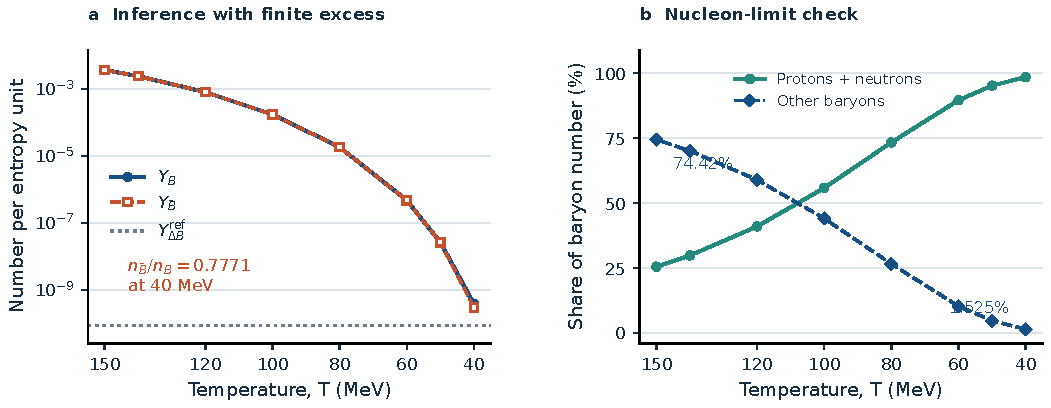
\includegraphics[width=.99\textwidth]{figures/fig05_inverse_en.pdf}
\caption{Our results addressing the retrospective objective. (a) Baryon and antibaryon yields inferred with PDG2025 and the published net excess as an input constraint. Curves nearly coincide at high temperature; their difference becomes a larger share of the total during cooling. The gray line is the conserved external constraint. (b) Shares of protons plus neutrons and of other baryons in the symmetric control. These shares were calculated here; the literature comparison uses the nucleon approximation of Satarov et al. (2013). Points are equilibrium states at specified temperatures rather than a measured kinetic trajectory.}
\label{fig:inverse}
\end{figure*}

\subsection{Quantities at alternative starting temperatures}
The 156.5-MeV transition reference corresponded to $1.8161\times10^{12}$ K. Under the same inverse conditions, PDG2025 yielded approximately $2.6575\times10^{37}$ baryons and the same rounded antibaryon density per cm$^3$. The excess was $4.8753\times10^{29}$ cm$^{-3}$, with $\mu_B/T=9.1749\times10^{-9}$. The total, $5.3150\times10^{37}$ cm$^{-3}$, exceeded the 150-MeV value by 54.31\%. Yield increased by 26.95\% to $9.4772\times10^{-3}$, distinguishing population and normalization changes. Table~\ref{tab:initialT} provides the sensitivity points. The 156.5-MeV result is our HRG evaluation at a published reference temperature, without turning it into a measured annihilation onset.

\begin{table*}[t]\centering\small
\caption{Our starting-temperature sensitivity using PDG2025 and the same net constraint. The transition reference is $156.5\pm1.5$ MeV (HotQCD, 2019); 150 MeV remains the main-grid start. The near-transition interval is neither a complete HRG uncertainty nor a measured annihilation onset.}\label{tab:initialT}
\setlength{\tabcolsep}{11pt}\renewcommand{\arraystretch}{1.14}
\begin{tabular}{rrrrr}\toprule
$T$ (MeV) & $n_B$ (${\rm cm^{-3}}$) & $n_{\bar B}$ (${\rm cm^{-3}}$) & $\Delta n_B$ (${\rm cm^{-3}}$) & $Y_\Sigma$ \\ \midrule
150 & $1.722\times10^{37}$ & $1.722\times10^{37}$ & $4.011\times10^{29}$ & 0.007465 \\
155 & $2.410\times10^{37}$ & $2.410\times10^{37}$ & $4.660\times10^{29}$ & 0.008991 \\
156.5 & $2.657\times10^{37}$ & $2.657\times10^{37}$ & $4.875\times10^{29}$ & 0.009477 \\
158 & $2.926\times10^{37}$ & $2.926\times10^{37}$ & $5.100\times10^{29}$ & 0.009976 \\
\bottomrule\end{tabular}\end{table*}


\subsection{Information recoverable from the present abundance}
The map in Eq.~\eqref{eq:rank} had rank one for two unknown components and null direction $(1,1)$. Four examples with totals of 0.1, 1, 10, and 100 times the initial total algebraically preserved $Y_B-Y_{\bar B}=8.6932\times10^{-11}$, equivalent to the same input $\eta=6.12\times10^{-10}$. The present excess alone therefore did not identify a unique initial pair population. Equilibrium at a specified temperature provided the additional information used in the reconstruction above.

\subsection{Quantitative comparison with the published nucleon limit}
Our evaluation of Eq.~\eqref{eq:nucleonMB} gave $n_p+n_n=4.4080\times10^{36}$ cm$^{-3}$ at 150 MeV in the Maxwell-Boltzmann approximation. The Fermi-Dirac sum was $4.4054\times10^{36}$ cm$^{-3}$, a relative difference of 0.05916\%. Nucleons supplied 25.5799\% of symmetric HRG baryon density; other baryons supplied 74.4201\%. At 40 MeV the nucleon share reached 98.4745\% (Table~\ref{tab:nucleoncontrast}). These numbers are our calculations using the stated approximation and catalog, rather than measured populations or values tabulated by the compared authors.

\begin{table*}[t]\centering\small
\caption{Calculated comparison with the nucleon limit of Satarov et al. (2013), generalized to distinct $p$ and $n$ masses. All numerical columns are our results at $\mu_B=0$. $\delta_{\rm MB}$ is $100(n_N^{\rm MB}/n_N^{\rm FD}-1)$; other-baryon share uses the full Fermi-Dirac HRG total.}\label{tab:nucleoncontrast}
\setlength{\tabcolsep}{8pt}\renewcommand{\arraystretch}{1.14}
\begin{tabular}{rrrrr}\toprule
$T$ (MeV) & $n_N^{\rm MB}$ (${\rm cm^{-3}}$) & $n_B^{\rm HRG}$ (${\rm cm^{-3}}$) & Other baryons (\%) & $\delta_{\rm MB}$ (\%) \\ \midrule
150 & $4.408\times10^{36}$ & $1.722\times10^{37}$ & 74.4201 & 0.05916 \\
140 & $2.498\times10^{36}$ & $8.354\times10^{36}$ & 70.1063 & 0.03814 \\
120 & $6.261\times10^{35}$ & $1.525\times10^{36}$ & 58.9552 & 0.01268 \\
100 & $9.612\times10^{34}$ & $1.720\times10^{35}$ & 44.1293 & 0.002696 \\
80 & $6.342\times10^{33}$ & $8.643\times10^{33}$ & 26.6153 & $2.623\times10^{-4}$ \\
60 & $7.938\times10^{31}$ & $8.859\times10^{31}$ & 10.3973 & $5.341\times10^{-6}$ \\
50 & $2.591\times10^{30}$ & $2.722\times10^{30}$ & 4.7824 & $2.357\times10^{-7}$ \\
40 & $1.664\times10^{28}$ & $1.690\times10^{28}$ & 1.5255 & $2.176\times10^{-9}$ \\
\bottomrule\end{tabular}\end{table*}


\subsection{Symmetric control of the initial inventory}
To check the effect of imposed symmetry, the calculation was repeated at $\mu_B=0$. The PDG2025 inventory supplied 443 active particle species: 146 baryonic, 146 antibaryonic, and 151 mesonic. These counts described particle types; populations were calculated using Eq.~\eqref{eq:number}. At $T_i=150$ MeV, our calculation gave
\begin{align}
n_B^{\rm eq}&=1.7222003\times10^{37}\ {\rm cm^{-3}},\\
n_{\bar B}^{\rm eq}&=1.7222003\times10^{37}\ {\rm cm^{-3}},\\
n_\Sigma^{\rm eq}&=3.4444006\times10^{37}\ {\rm cm^{-3}}.
\label{eq:initialpopulation}
\end{align}
For each physical cm$^3$ of plasma at this temperature, the reconstructed mean number was $1.7222\times10^{37}$ baryons and the same number of antibaryons. Symmetric bookkeeping corresponded to $1.7222\times10^{37}$ potential pairs per cm$^3$. Meson and photon densities were $2.4649\times10^{38}$ and $1.0700\times10^{38}$ cm$^{-3}$, respectively.

For nucleonic particle species we obtained $n_p=n_{\bar p}=2.2103\times10^{36}$ and $n_n=n_{\bar n}=2.1951\times10^{36}$ cm$^{-3}$. Protons and neutrons jointly supplied 25.58\% of all baryons in the inventory at 150 MeV. These were primary equilibrium populations before resonance-decay feed-down. The identity $n_B=n_{\bar B}$ gave zero net excess in the symmetric control.

\subsection{Symmetric-control abundance sequence during cooling}
Table~\ref{tab:populations} lists the reconstruction at all eight temperatures. At 40 MeV we obtained $n_B=n_{\bar B}=1.6896\times10^{28}$ cm$^{-3}$ and $n_\Sigma=3.3791\times10^{28}$ cm$^{-3}$. Total yield decreased from $Y_\Sigma^{\rm eq}=7.4653\times10^{-3}$ to $6.8756\times10^{-10}$, a reduction of 7.0357 orders of magnitude (Fig.~\ref{fig:populations}). Physical number per cm$^3$ and yield per entropy unit were retained as distinct quantities.

\begin{table*}[t]\centering\small
\caption{Equilibrium number densities reconstructed with PDG2025 at zero chemical potentials. The second column gives the density of each side; the total includes both. $Y_\Sigma=n_\Sigma/s_{\rm tot}$ separates thermal suppression from dilution. $\mathcal Q=Y_\Sigma/Y_{\Delta B}^{\rm ref}$ uses the cosmic excess as an external input. These are calculated instantaneous populations, without counting regeneration or annihilation events.}\label{tab:populations}
\setlength{\tabcolsep}{12pt}\renewcommand{\arraystretch}{1.14}
\begin{tabular}{rrrrr}\toprule
$T$ (MeV) & $n_B=n_{\bar B}$ (${\rm cm^{-3}}$) & $n_\Sigma$ (${\rm cm^{-3}}$) & $Y_\Sigma$ & $\mathcal Q$ \\ \midrule
150 & $1.722\times10^{37}$ & $3.444\times10^{37}$ & 0.007465 & $8.587\times10^{7}$ \\
140 & $8.354\times10^{36}$ & $1.671\times10^{37}$ & 0.004887 & $5.622\times10^{7}$ \\
120 & $1.525\times10^{36}$ & $3.051\times10^{36}$ & 0.001634 & $1.880\times10^{7}$ \\
100 & $1.720\times10^{35}$ & $3.441\times10^{35}$ & $3.506\times10^{-4}$ & $4.033\times10^{6}$ \\
80 & $8.643\times10^{33}$ & $1.729\times10^{34}$ & $3.687\times10^{-5}$ & $4.241\times10^{5}$ \\
60 & $8.859\times10^{31}$ & $1.772\times10^{32}$ & $9.595\times10^{-7}$ & $1.104\times10^{4}$ \\
50 & $2.722\times10^{30}$ & $5.443\times10^{30}$ & $5.331\times10^{-8}$ & 613.2 \\
40 & $1.690\times10^{28}$ & $3.379\times10^{28}$ & $6.876\times10^{-10}$ & 7.909 \\
\bottomrule\end{tabular}\end{table*}

\begin{figure*}[t]
\centering
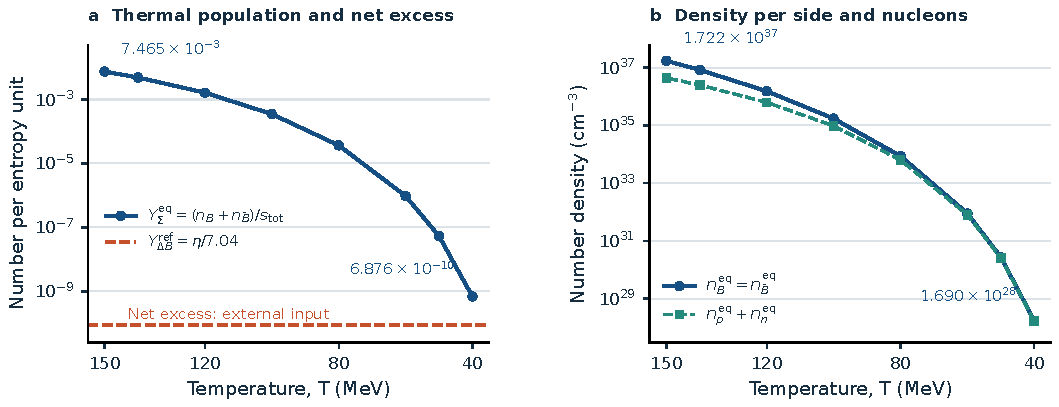
\includegraphics[width=.99\textwidth]{figures/fig04_populations_en.pdf}
\caption{Our reconstruction of number populations using PDG2025. (a) Total thermal yield $Y_\Sigma^{\rm eq}$ and reference net excess $Y_{\Delta B}^{\rm ref}=8.6932\times10^{-11}$. The net-excess line uses an external cosmic normalization; the blue curve was calculated from the HRG inventory. (b) Density of each symmetric side and the proton-plus-neutron contribution. Each antiparticle curve coincides with its particle counterpart in the symmetric control. Axes follow cooling and segments guide the eye. These are instantaneous equilibrium populations, without counting cumulative annihilation or regeneration events.}
\label{fig:populations}
\end{figure*}


\subsection{Comparison at fixed temperature}
All three larger lists produced fractions that decreased throughout the temperature grid during cooling (Table~\ref{tab:comparison}; Figure~\ref{fig:comparison}). PDG2025 yielded
\begin{align}
\fB(150\ {\rm MeV})&=0.08454533,\\
\fB(40\ {\rm MeV})&=1.7970078\times10^{-8}.
\end{align}
The first value is 8.4545\%, whereas the second is $1.7970\times10^{-6}\%$.

\begin{table*}[t]\centering\footnotesize
\caption{Comparison at fixed temperature of the baryon-antibaryon entropy fraction. The four $f$ columns are dimensionless fractions; the last two are percentages. The reduced reference was transcribed from the prior manuscript; the PDG columns were calculated in this audit with the same light plasma. The descriptive ratio was evaluated before rounding the PDG result.}\label{tab:comparison}
\setlength{\tabcolsep}{9pt}\renewcommand{\arraystretch}{1.14}
\begin{tabular}{rrrrrrr}\toprule
$T$ (MeV) & $f_{\mathrm{prior}}$ & $f_{\mathrm{PDG2014}}$ & $f_{\mathrm{PDG2020}}$ & $f_{\mathrm{PDG2025}}$ & $100R$ & $100d$ \\ \midrule
150 & 0.06208 & 0.08351 & 0.08459 & 0.08455 & 73.43 & 26.57 \\
140 & 0.04328 & 0.05633 & 0.05695 & 0.05693 & 76.02 & 23.98 \\
120 & 0.01686 & 0.02018 & 0.02032 & 0.02032 & 82.97 & 17.03 \\
100 & 0.004305 & 0.004734 & 0.00475 & 0.00475 & 90.64 & 9.36 \\
80 & $5.464\times10^{-4}$ & $5.655\times10^{-4}$ & $5.661\times10^{-4}$ & $5.661\times10^{-4}$ & 96.52 & 3.48 \\
60 & $1.782\times10^{-5}$ & $1.795\times10^{-5}$ & $1.795\times10^{-5}$ & $1.795\times10^{-5}$ & 99.26 & 0.74 \\
50 & $1.148\times10^{-6}$ & $1.152\times10^{-6}$ & $1.152\times10^{-6}$ & $1.152\times10^{-6}$ & 99.67 & 0.33 \\
40 & $1.795\times10^{-8}$ & $1.797\times10^{-8}$ & $1.797\times10^{-8}$ & $1.797\times10^{-8}$ & 99.89 & 0.11 \\
\bottomrule\end{tabular}\end{table*}

\begin{figure*}[t]
\centering
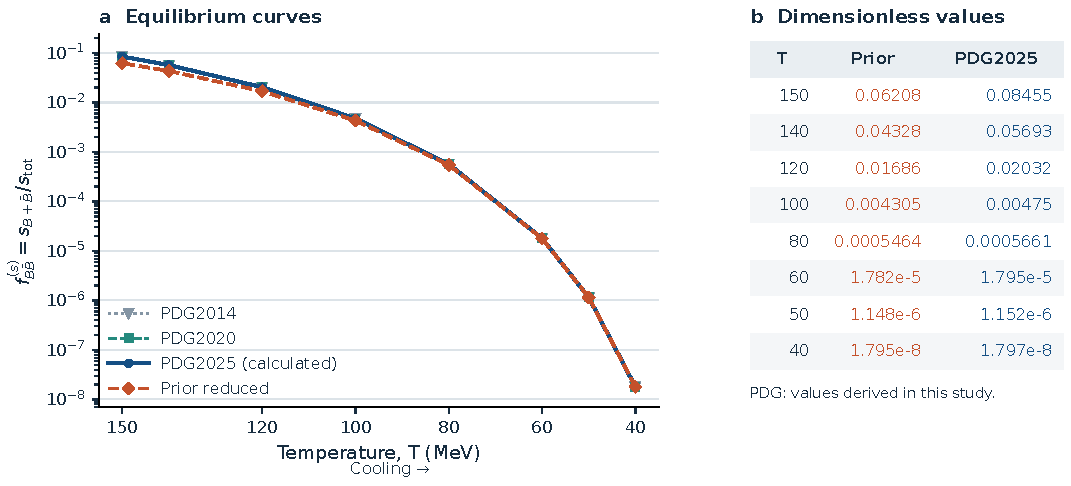
\includegraphics[width=.99\textwidth]{figures/fig01_comparison_en.pdf}
\caption{Baryon-antibaryon entropy fraction at vanishing chemical potentials. (a) Semilogarithmic comparison of the reduced reference with three independent calculations using Thermal-FIST lists based on PDG2014, PDG2020, and PDG2025. The horizontal axis follows cooling from left to right. (b) Dimensionless values of the reference and the PDG2025 calculation at all eight temperatures. Every PDG curve is a result derived in this calculation, with zero resonance widths and a common light sector in the denominator, rather than an external measurement. Segments connect calculated points as visual guides.}
\label{fig:comparison}
\end{figure*}

At 150 MeV, the prior reference of 6.208\% lay 2.2465 percentage points below the PDG2025 calculation. The ratio $R$ was 0.73428 and the relative deficit was 26.57\%. During cooling, $100R$ increased to 90.64\% at 100 MeV, 99.26\% at 60 MeV, and 99.89\% at 40 MeV (Figure~\ref{fig:convergence}). The maximum spread across lists on the grid occurred at 150 MeV: 0.10775 percentage points. Their percentages there were 8.3509, 8.4586, and 8.4545\% for PDG2014, PDG2020, and PDG2025, respectively.

\begin{figure*}[t]
\centering
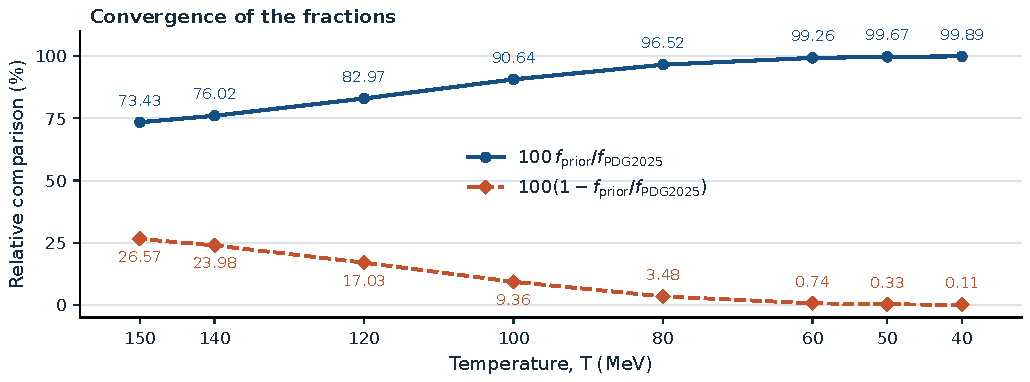
\includegraphics[width=.99\textwidth]{figures/fig02_convergence_en.pdf}
\caption{Relative contrast between the prior reduced reference and the PDG2025 calculation. Blue points show $100R=100f_{\rm prior}/f_{25}$; orange points show its complement, $100d=100(1-R)$. Labels report percentages calculated before rounding $f_{25}$, using the four significant digits available for the prior reference. These quantities measure numerical agreement between equilibrium fractions; they are neither validation probabilities nor percentages of annihilated pairs.}
\label{fig:convergence}
\end{figure*}

\subsection{Shape of the series}
Correlation between the logarithms of the eight fractions was $r_{\log}=0.9999233$, with $\mathrm{RMSE}_{\log}=0.0714338$. The endpoint ratio was $2.89143\times10^{-7}$ for the reduced reference and $2.12550\times10^{-7}$ for PDG2025. Corresponding decreases were 6.539 and 6.673 orders of magnitude. Spearman's rank correlation was $\rho_S=1$, consistent with the common monotonic ordering. These metrics summarized series shape and amplitude differences on the selected grid.

\subsection{Densities and denominator effect}
PDG2025 at 150 MeV gave the following densities:
\begin{align}
\sB&=2.9972147\times10^{-3}\ {\rm GeV^3},\\
s_{\rm mes}&=1.1626411\times10^{-2}\ {\rm GeV^3},\\
\shad&=1.4623626\times10^{-2}\ {\rm GeV^3},\\
\sL&=2.0827352\times10^{-2}\ {\rm GeV^3},\\
\stot&=3.5450978\times10^{-2}\ {\rm GeV^3}.
\end{align}
The partition of $\stot$ was 8.4545\% baryons and antibaryons, 32.7957\% mesons, and 58.7497\% light sector. Using $\shad$ alone as the denominator gave 20.4957\% for the same numerator (Figure~\ref{fig:denominator}).

\begin{figure*}[t]
\centering
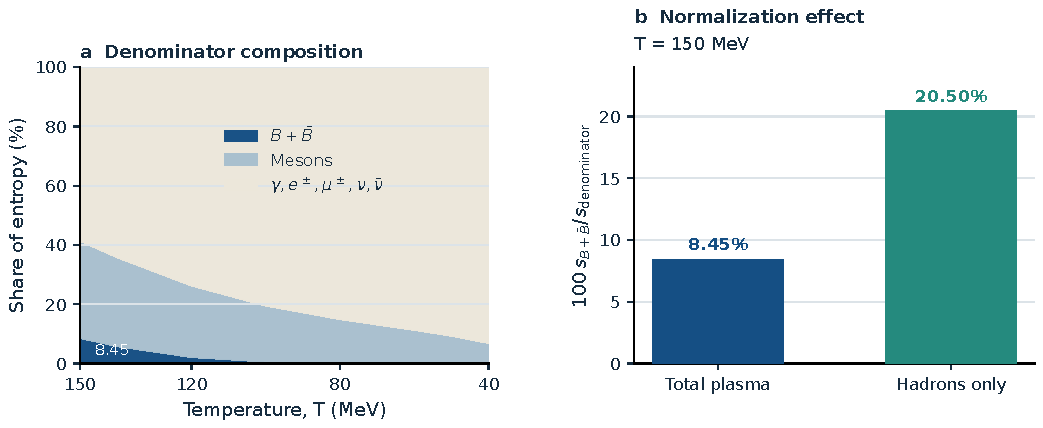
\includegraphics[width=.99\textwidth]{figures/fig03_denominator_en.pdf}
\caption{Effect of the total-entropy definition in the PDG2025 calculation. (a) Shares of baryons and antibaryons, mesons, and the light sector in $\stot$ at all eight temperatures; areas between points are visual guides. (b) The same numerator $\sB$ at 150 MeV represents 8.45\% of the entropy of the selected plasma and 20.50\% of exclusively hadronic entropy. The change reflects normalization rather than a different baryonic population. The figure describes instantaneous equilibrium composition, without identifying the individual fate of annihilation products.}
\label{fig:denominator}
\end{figure*}

\subsection{Relic scale and connection with H and He}
Normalization to the external excess $\YB^{\rm ref}=8.6932\times10^{-11}$ gave $\mathcal Q(150)=8.5875\times10^7$ and $\mathcal Q(40)=7.9092$. Per reference unit of net baryon number, the initial symmetric population represented $4.2937\times10^7$ baryons and the same number of antibaryons. This comparison used a common comoving normalization. At 40 MeV the symmetric equilibrium total remained 7.91 times that excess; the grid endpoint was not a calculated final relic.

Observational inputs and Eqs.~\eqref{eq:today} and \eqref{eq:hydrogen} gave Table~\ref{tab:present}. The inferred mean baryon density was $(2.514\pm0.017)\times10^{-7}$ cm$^{-3}$, or $0.2514\pm0.0017$ baryon-number units per m$^3$. Within input rounding, this agreed with the reference $(2.515\pm0.017)\times10^{-7}$ cm$^{-3}$ compiled by \citet{Groom2025}. Both conversions shared the CMB normalization.

\begin{table}[t]
\centering\small
\caption{Conversions calculated from published cosmological inputs. Uncertainties use first-order input propagation, excluding HRG physical uncertainties. H, He, and D denote a primordial-composition equivalent at today's mean density, rather than a census of present neutral atoms.}
\label{tab:present}
\setlength{\tabcolsep}{3pt}\renewcommand{\arraystretch}{1.18}
\begin{tabular}{lr}\toprule
Quantity & Density (${\rm cm^{-3}}$)\\\midrule
CMB photons & $410.73\pm0.27$\\
Net baryon number & $(2.514\pm0.017)\times10^{-7}$\\
H nuclei & $(1.898\pm0.015)\times10^{-7}$\\
$^4$He nuclei & $(1.540\pm0.021)\times10^{-8}$\\
D nuclei & $(4.760\pm0.066)\times10^{-12}$\\
\bottomrule\end{tabular}
\end{table}

The retrospective sequence was: present abundance, conservation constraint on net yield, HRG inventory properties, specified temperature, and solution for early populations. H/He/D conversions described the cosmological reference used, rather than independent HRG predictions.

\subsection{Numerical and chemical checks}
Number-density quadrature and series differed by less than $5\times10^{-16}$ at recorded precision. We exported 3544 records for 443 particle species at eight temperatures.

Doubling the series length did not change the fractions at the recorded arithmetic precision. Independent integrals met the $10^{-8}$ criterion for all tested species and temperatures. The massless-electron approximation overestimated electron entropy by relative amounts of $1.26\times10^{-6}$ at 150 MeV and $1.77\times10^{-5}$ at 40 MeV.

The inverse solution closed the net constraint with a maximum relative error of $2.23\times10^{-15}$ across the three lists. Changes on doubling the number of terms were below $4.5\times10^{-16}$. Independent nucleon-excess integrals agreed with the sums within a relative $3.83\times10^{-13}$. At 40 MeV, the finite excess increased total baryon-plus-antibaryon density by 0.7961\% relative to the symmetric control. Validation files distinguished this reconstruction from zero-potential checks.
